% ------------------------------------------------------------
% LaTeX Template für die DHBW zum Schnellstart!
% Original: https://github.wdf.sap.corp/vtgermany/LaTeX-Template-DHBW
% ------------------------------------------------------------
% ---- Präambel mit Angaben zum Dokument
\input{Inhalt/00_Latex/praeambel}

% ---- Elektronische Version oder Gedruckte Version?
% ---- Unterschied: Die elektronische Version enthält keinen Platzhalter für die Unterschrift
\usepackage{ifthen}
\newboolean{e-Abgabe}
\setboolean{e-Abgabe}{false}    % false=gedruckte Fassung

% ---- Persönlichen Daten:
\newcommand{\titel}{Enhancing insights into spending through aggregation with automated document clustering of a large-scale multilingual corpus}
\newcommand{\titelheader}{ }
\newcommand{\arbeit}{Bachelor Thesis}
\newcommand{\studiengang}{Internationale Wirtschaftsinformatik}
\newcommand{\studienjahr}{2019}
\newcommand{\autor}{Lisa Schmidt}
\newcommand{\autorReverse}{Schmidt, Lisa}
\newcommand{\verfassungsort}{Ludwigshafen}
\newcommand{\matrikelnr}{631971}
\newcommand{\kurs}{IBAIT19}
\newcommand{\bearbeitungsmonat}{Januar 2018}
\newcommand{\abgabe}{01. Februar 2018}
\newcommand{\bearbeitungszeitraum}{01.10.2017 - 31.01.2018}
\newcommand{\firmaName}{SAP SE}
\newcommand{\firmaStrasse}{Dietmar-Hopp-Allee 16}
\newcommand{\firmaPlz}{69190 Walldorf, Deutschland}
\newcommand{\betreuerFirma}{Dr. Karthik Muthuswamy}
\newcommand{\betreuerDhbw}{Prof. Dr. Joachim Melcher}

\input{Inhalt/00_Latex/kopfundFusszeile}

% ---- Hilfreiches
\newcommand{\zB}{z.\,B. }   % "z.B." mit kleinem Leeraum dazwischen (ohne wäre nicht korrekt)
\newcommand{\dash}{d.\,h. }

\newcommand{\code}[1]{\texttt{#1}} % Ist einfacher zu schreiben als ständig \texttt und erlaubt
                                   % Änderungen im Nachhinein, wenn man z.B. Inline-Code anders stylen möchte.

% ---- Silbentrennung (falls LaTeX defaults falsch / nicht gewünscht sind)
\hyphenation{HANA}         % anstatt HA-NA
\hyphenation{Graph-Script} % anstatt GraphS-cript

% ---- Beginn des Dokuments
\begin{document}
\setlength{\parindent}{0pt}              % Keine Paragraphen Einrückung.
                                         % Dafür haben wir den Abstand zwischen den Paragraphen.
\setcounter{secnumdepth}{2}              % Nummerierungstiefe fürs Inhaltsverzeichnis
\setcounter{tocdepth}{1}                 % Tiefe des Inhaltsverzeichnisses. Ggf. so anpassen,
                                         % dass das Verzeichnis auf eine Seite passt.
\sffamily                                % Serifenlose Schrift verwenden.

% ---- Vorspann
% ------ Titelseite
\singlespacing
\thispagestyle{empty}
\begin{titlepage}
\enlargethispage{4cm}

\begin{figure}           % Logo vom Ausbildungsbetrieb und der DHBW
	% \vspace*{-5mm} % Sollte dein Titel zu lang werden, kannst du mit diesem "Hack" 
	%                  den Inhalt der Seite nach oben schieben.
	\begin{minipage}{0.49\textwidth}
		\flushleft
		%\includegraphics[height=2.5cm]{Bilder/Logos/Logo_SAP.pdf} 
	\end{minipage}
	\hfill
	\begin{minipage}{0.49\textwidth}
		
		%\includegraphics[height=2cm]{Bilder/Logos/Logo_HWGLU.png} 
	\end{minipage}
	\hfill
\end{figure} 
\vspace*{0.1cm}

\begin{center}
	\huge{\textbf{\titel}}\\[1.5cm]
	\Large{\textbf{\arbeit}}\\[0.5cm]
	\normalsize{Part of the Examination for the\\[1ex] \textbf{Bachelor of Science (B.Sc.)}}\\[0.5cm]
	\Large{of \studiengang}\\[1ex]
	\normalsize{at the University of Business and Society Ludwigshafen}\\[1cm]
	\normalsize{by}\\[1ex] \Large{\textbf{\autor}} \\[1cm]
	% Hinweis: Manche Dozenten möchten einen Hinweis auf den Sperrvermerk auf der Titelseite.
	% \large{{\color{red}- Sperrvermerk -}}\\[1cm]
\end{center}

\begin{center}
	\vfill
	\begin{tabular}{ll}
		Date of submission:                     & \abgabe \\[0.2cm]
		Timeframe:            & \bearbeitungszeitraum \\[0.2cm]
		Matriculation Number, Kurs:            & \matrikelnr , \kurs \\[0.2cm]
		Company:                & \firmaName \\
		                                 & \firmaStrasse \\
		                                 & \firmaPlz \\[0.2cm]
		Company Supervisor:   & \betreuerFirma \\[0.2cm]
		Academic Supervisor: & \betreuerDhbw \\[2cm]
	\end{tabular} 
\end{center}
\end{titlepage}
  % Titelseite
\newcounter{savepage}
\pagenumbering{Roman}                    % Römische Seitenzahlen
\onehalfspacing

% ------ Erklärung, Sperrvermerk, Abstact
%\chapter*{Statutory Declaration}

I hereby declare that this Bachelor thesis 

\begin{quote}
	\textit{\titel}
\end{quote} 

represents my original work and that I have used no other sources except as noted by citations. All data, tables, figures and text citations which have been reproduced from any other source, including the internet, have been explicitly acknowledged as such. This thesis has not been presented, so far, in the same or similar form in any other study course as examination performance or otherwise published.

Additionally, I certify that the printed version is identical to the electronic document.

\vspace{1cm}

\verfassungsort, June 1, 2022 \\[0.5cm]
\ifthenelse{\boolean{e-Abgabe}}
	{\underline{Gez. \autor}}
	{\makebox[6cm]{\hrulefill}}\\ 
\autorReverse

%\chapter*{Restriction Notice}

This Bachelor thesis contains strictly confidential information and business secrets of SAP SE. It is exclusively provided as an examination submission. Disclosure of information to anyone other than the examination board or lectors is not authorized. Copying, quoting, duplicating or publishing is not allowed without the explicit written authorization of SAP SE.

%\include{Inhalt/02_Abstract/abstract-en}
%\include{Inhalt/02_Abstract/abstract-de}

% ------ Inhaltsverzeichnis
\singlespacing
\setcounter{tocdepth}{10}
\tableofcontents

% ------ Verzeichnisse
\renewcommand*{\chapterpagestyle}{plain}
\pagestyle{plain}
%\include{Inhalt/03_Verzeichnisse/formelgroessen}
\chapter*{List of Abbreviations}
\addcontentsline{toc}{chapter}{List of Abbreviations} % Hinzufügen zum Inhaltsverzeichnis 

\begin{acronym}[WYSISWG] % längstes Kürzel wird verw. für den Abstand zw. Kürzel u. Text

	% Alphabetisch selbst sortieren - nicht verwendete Kürzel rausnehmen!
	\acro{AI}{Artificial Intelligence}
	\acro{BERT}{Bidirectional Encoder Representations from Transformers}
	\acro{BoW}{Bag of Words}
	\acro{CPU}{Central Processing Unit}
	\acro{CRISP-DM}{Cross Industry Standard Process for Data Mining}
	\acro{CoE}{Center of Excellence}
	\acrodefplural{CoE}{Centers of Excellence}
	\acro{DBSCAN}{Density-based Spatial Clustering of Applications with Noise}
	\acro{DR}{Dimensionality Reduction}
	\acro{ERP}{Enterprise Resource Planning}
	\acro{FFNN}{Feed-Forward Neural Network}
	\acro{GPU}{Graphics Processing Unit}
	\acro{JSON}{JavaScript Object Notation}
	\acro{KDD}{Knowledge Discovery in Databases}
	\acro{ML}{Machine Learning}
	\acro{NLP}{Natural Language Processing}
	\acro{NLTK}{Natural Language Toolkit}
	\acro{PCA}{Principal Component Analysis}
	\acro{SEMMA}{Sample Explore Modify Model Assess}
	\acro{sklearn}{scikit-learn}
	\acro{SQL}{Short Query Language}
	\acro{TF-IDF}{Term Frequency - Inverse Document Frequency}	
	\acro{t-SNE}{T-Distributed Stochastic Neighbor Embedding}
	\acro{TPU}{Tensor Processing Unit}


\end{acronym}
\listoffigures                          % Erzeugen des Abbildungsverzeichnisses 
\listoftables                           % Erzeugen des Tabellenverzeichnisses
%\renewcommand{\lstlistlistingname}{Quellcodeverzeichnis}
\lstlistoflistings                      % Erzeugen des Listenverzeichnisses
%\setcounter{savepage}{\value{page}}


% ---- Inhalt der Arbeit
\cleardoublepage
\pagenumbering{arabic}                  % Arabische Seitenzahlen für den Hauptteil
\setlength{\parskip}{0.5\baselineskip}  % Abstand zwischen Absätzen
\rmfamily
\renewcommand*{\chapterpagestyle}{scrheadings}
\pagestyle{scrheadings}
\onehalfspacing
% \include{Inhalt/04_Inhalt/einleitung}
%\include{Inhalt/04_Inhalt/formatText}
% \include{Inhalt/04_Inhalt/abbildungen}
%\include{Inhalt/04_Inhalt/mathematische-formeln}
%\include{Inhalt/04_Inhalt/quellcode}
%\include{Inhalt/04_Inhalt/literaturHinweis}

\chapter{Introduction}
\section{Motivation}

More than 4 out of 5 financial departments are "overwhelmed by the high numbers of invoices they are expected to process"  \cite{manualInvoiceProcessing}. Already swamped departments struggle with providing information on savings potential. A solution for processing large amounts of invoice data with minimal human interference is desirable. Processing this information should transform unstructured data into a useful format, further the data should be enriched in a way giving insight and provide value for financial advisors. With analysis results of this automated processing, financial advisors can enjoy two improvements. Firstly, they have a factual base for recommendations. Secondly, their financial department is able to focus on more value-adding tasks. If an automated solution completes the time-consuming task of an in-depth analysis of spending, more time is available for interpreting the results.

In general, internal financial reporting aims to provide information about the health of a company, and supply means for improvement. Invoices are the main source of information for controlling \cite{investopediaInvoices}, as they record the complete history of cash flow \cite{invoicesPurpose}. An invoice is a document recording the main information on a sales transaction. Usually, an invoice contains the unit cost, a timestamp, and payment terms. Other information, such as shipping terms, shipping address, or discounts may also be included. 

\section{Current Situation}
An essential part of economic counseling is the assessment of spending for different company segments. Spending of a firm usually is written down in invoice documents, which have to be grouped  to analyze cost types.
The global market is estimated to comprise 550 billion invoices annually, but 90\% are exchanged paper-based \cite[p.~5]{kochEInvoicingJourney}. With modern technology, these paper-based or digital documents can be transformed into a structured or semi-structured format. According to expert estimates, unstructured data makes up for more than 80\% of enterprise data \cite{structuredAndUnstructuredData}. Companies can not utilize unstructured data to its full potential, as this data is not able to be leveraged with traditional data analysis tools.

\section{Research Questions}
\label{section:research-q}
How can information from invoice-like documents be extracted?
How can extracted information provide insights?

\section{Outline}
The introductory chapter briefly explains the motivation behind the thesis. Also, it assesses the current situation and presents research questions. Lastly, it presents the structure of the thesis.

The following Chapter about objectives and criteria gives a detailed task description, and establishes criteria. In Section \ref{research-model}, the process model is explained, evaluated and adjusted.

Chapter 3 sheds light on the corporate environment with respect to the aspects of history and organization.

Chapter 4 explains the process of selecting a dataset. The chapter presents fundamental types of projects and data sources, as well as decision-relevant criteria. With these criteria in mind, the chapter presents the selected dataset.

Chapter 5 explains the business dimension of the task by presenting all relevant business and technical terms in a glossary. The chapter sets objectives and goals, while also proposing different measures to contains risks.
Additionally, the chapter puts forward an initial assessment of tools and techniques.

Chapter 6 explains the data by visualizing different aspects in the dataset. After exploring the data, Chapter 6 also measures the data quality.

In Chapter 7, the preparation of the data is explained. The processes of data wrangling and feature extraction are illustrated with an extensive evaluation of alternatives, a theoretical, and a practical implementation of the solution. Further, the chapter details the task of cleaning the data.

Chapter 8 concerns the use of a machine learning model to cluster the data. By presenting different measures, algorithms and models, the chapter presents a careful evaluation of alternatives. Further, the chapter displays the planned implementation and the results of the practical implementation.

Chapter 9 describes the deployment of the solution.

Chapter 10 presents the evaluation of the result. The Chapter evaluates the output from the previous steps.

In Chapter 11, a conclusion is drawn, and a further outlook is given.
\chapter{Objectives and Criteria}
\section{Detailed Task Description}
\section{Criteria set by SAP SE}
\chapter{Fundamentals}
\section{Glossary of Terms}

\section{Corporate Environment}
\section{SAP AI Core}



\chapter{Dataset selection}

	\section{Choosing a Data Source}
	\label{data-source}
	
	With the project type as a decisive factor for the dataset explained, the other evaluation criteria for the dataset is described. In the corporate environment two fundamental sources for data exist. 
	
	\begin{table}[]
		\caption{Comparison of Data Sources}
		\begin{tabular}{lll}
			\toprule
			 & \textbf{Internal Data}                                                                                             & \textbf{External Data}                                                                                               \\
			\midrule
			
			Source       & \begin{tabular}[c]{@{}l@{}}Internal or customer data, \\ bought or generated\end{tabular}            & \begin{tabular}[c]{@{}l@{}}Publicly available, \\ generated or supplied by companies\end{tabular}      \\ \midrule
			
			Relevance    & Business-relevant                                                                                    & Anonymized, processed                                                                                  \\ \midrule
			
			Value        & Relevant specific business                                                                           & Of general relevance                                                                                   \\ \midrule
			
			Availability & \begin{tabular}[c]{@{}l@{}}Authorization processes in place,\\ data protection measures\end{tabular} & Ubiquitously available                                                                                 \\ \midrule
			Examples     & \begin{tabular}[c]{@{}l@{}}Sales records, usage statistics, \\ customer feedback\end{tabular}        & \begin{tabular}[c]{@{}l@{}}Historic weather information, con- \\  sumer statistics, social media data\end{tabular}\\
			\bottomrule
		\end{tabular}
	\end{table}
	
	\subsection{Potential Data Sources}
	Firstly, data can be sourced from inside the company. This can include customer data or data generated from observation and monitoring processes inside the company \cite{internalExternalData}. Data is either directly or very closely related to the company's business. Because internally sourced data is of utter utility and a possible target for industrial espionage, internally sourced data is almost exclusively rated confidential, limiting even intra-company access to it. Authorization processes and more than often not existing registries for data may hinder project progress.
	
	Secondly, data can be sourced outside the company. A vast number of online registries for data exist, both with paid and free of charge service offerings \cite{whyExternalData}. Data sources include social media data, sensory data and weather data. Because of its publication, the data is sometimes stripped from all parts which could expose confidential information such as corporate secrets. Additionally, data is anonymized for privacy reasons. External Data can give valuable insights into industries and markets especially for data scientists without access to paid databases, or for small businesses without the option for an own data collection.
	
	
	
	\subsection{Selected Data Source}
	It can be stated, that both sources are suited for different goals and different contexts. For data scientists with internal sources available, this type of source seems more appealing. An approach of connecting both internal and external data is an option, but not within the scope of this project. For this project, internally sourced data is chosen as a source.
	
	\section{Choosing a Dataset}
	The dataset is the foundation of a data-science project. The quality, size, and closeness to reality decide the helpfulness of findings made using the data.
	In this section, a classification for data-science projects is introduced as a guide for dataset selection.
	
	\subsection{Project Types}
\begin{table}[ht]
	\caption{Fundamental Data Science Project Types}
	\begin{tabular}{lll}
		\toprule
		& \textbf{Problem-First}                                                                                                              & \textbf{Data-First}                                                                                                                                                \\
		\midrule
		
		Systematics                                                             & Applied Data Science                                                                                                                & Exploratory Data Science                                                                                                                                           \\ \midrule
		\vspace{0.5cm}
		\begin{tabular}[c]{@{}l@{}}Underlying\\ Question\end{tabular}           & \begin{tabular}[c]{@{}l@{}}How can a problem be \\ solved?\end{tabular}                                                             & \begin{tabular}[c]{@{}l@{}}Which problems can be \\ solved with the solution?\end{tabular}                                                                         \\ \midrule
		\begin{tabular}[c]{@{}l@{}}Role of the \\ dataset\end{tabular}          & \begin{tabular}[c]{@{}l@{}}Different datasets can be \\ considered for one \\ problem statement\end{tabular}                       & \begin{tabular}[c]{@{}l@{}}The dataset is the core of \\ the project, with a new \\ dataset, a new project begins\end{tabular}                                    \\ \midrule
		\begin{tabular}[c]{@{}l@{}}Requirements \\ for the dataset\end{tabular} & \begin{tabular}[c]{@{}l@{}}Require a ground truth or \\ established methods for \\ evaluating the goal \\ achievement\end{tabular} & \begin{tabular}[c]{@{}l@{}}Compared to problem-first projects, \\ larger datasets are required because\\ there is no prior assumption of \\ patterns\end{tabular} \\ \midrule
		Fixed component                                                         & Problem statement                                                                                                                  & Dataset                                                                                                                                                           \\ \midrule
		Innovative Aspect                                                       & \begin{tabular}[c]{@{}l@{}}Defined during formu-\\ lation of the goal\end{tabular}                                                 & Found during the project                 \\
		\bottomrule                                                                                                                        
	\end{tabular}
\end{table}

	The problem-first project type is characterized by a predefined problem statement or research goal. The underlying question is how a specific problem can be solved \cite[p.~3051]{dataScienceProjectTypes}.  For the selection of the dataset, this requires that goal achievement can be measured with existing ground truth. In some cases, also other methods such as expert judgments can be sufficient. In a problem-first project different datasets can and should be considered. \cite[p.~3051]{dataScienceProjectTypes} give the metaphor of "mining for valuable minerals or metals at a given geographic location where the existence of the minerals or metals has been established". This means that it is already verified that the business goal can be reached with this specific dataset, hence the metaphor of already discovered mineral occurrence.
	
	The complementary project type is the data-first project. This type is characterized by a more exploratory approach, and the goal to find problems and patterns. Here, the dataset is at the core of the project and the fixed aspect of the project. In turn, this means swapping the dataset is the start of a new project. When turning to the metaphor of mining for minerals, this type of project would be the exploration of different test pits that promise mineral occurrences \cite[p.~3051]{dataScienceProjectTypes}. It is not clear if a problem can be solved with the investigation, and problem to solve is not known.
	
	\subsection{Systematization of this Project}
	Usually, the project type is not decided on, but implicitly arises out of environmental parameters. The goal of the analysis is clearly stated in before chapters. Still, the research questions (\ref{section:research-q}) aim at finding out which insights the analysis can give. Therefore, this project can be classified as a data-first project.
	
	\subsection{Resulting Requirements for Selecting a Dataset}
	In a data-first project, there is no assumption of patterns. This for once means that a large dataset is required to cover enough ground for accurate derivation of insights. Second, a data-first project does not require structured data \cite{srivastavaDataMining}. Instead, unstructured and semi-structured data is also applicable for data-first projects.
	
	
	\section{Selected Dataset}
	With the requirements explained, a dataset fulfilling all criteria was found. The selected document dataset consists of 150.000 invoices. The data contains information about the vendors, billing amounts and a descriptions of the goods. 
	
	

\chapter{Business Understanding}
In the guide complementing the \ac{CRISP-DM} model, different tasks, and outputs for developing a business understanding are mentioned. The task and respective output will be discussed in the following sections.

\section{Business Objectives}
\label{section:business-objectives}
Businesses without existing an \ac{ERP} solution in place can easily be overwhelmed by the number of invoices reaching them daily. Even more, the controlling department can easily lose the overview of spending. To quickly gain a perspective on the most important spending topics, spending should be sorted in categories of similar nature.

The primary goal is the development of a solution for automatic aggregation of documents, based on topics addressed in those documents. The focus is on shorter text segments, such as product descriptions. The business objective is an information gain, on how spending is distributed among cross-cutting topics in a company.

The created solution can be evaluated with the business success criterion: "Does the solution identify and give useful insights in the money pits?". The judgment of goal achievement is a subjective matter. Evaluating the success should therefore be distributed among several stakeholders, including but not limited to the author, the supervisor and the supplier of the data.

\section{Assessment of the Situation}

\subsection{Inventory of Resources}
An inventory of resources (\ref{tabelle:inventory}) was created for assessing the situation. Most notably is the availability of experts through excellent inter-corporation cooperation. Also, a large collection of datasets is available. Hardware platforms include personal machines as well as hosted environments with GPU capabilities. Available software are data science tools included in the Anaconda Navigator, such as Jupyter Notebook. All open-source libraries are of course also included.

\subsection{Requirements, Assumptions, and Constraints}
The project is to be completed the latest on June 7$^{th}$ 2022. 

Several assumptions underlay the process of data mining. First, it is assumed that the descriptions of the invoices is speaking enough to identify the product referenced.
Second, the analysis assumes that invoices can be logically grouped into clusters, in other words, several invoices referring to similar topics.

From a legal perspective, the project is constrained in the publication of data. While the use and processing of the supplied data is permitted within the context of the thesis, publication and further use is prohibited. The dataset is to be kept only on the local machine and SAP owned hyperscaler instances.

\subsection{Risks and Contingencies}
\paragraph{Dataset too Large for Processing} One specific risk that may arise in this project, is a dataset too large to be processed. Only a limited size of data is able to be loaded into memory. If the dataset turns out to be too big, four solutions are proposed.

\begin{enumerate}
	\item The dataset can be compressed using either a lossy compression (sampling, truncating floating point values) or a lossless compression (choosing only specific columns, using a sparse-column representation or choosing efficient data types) \cite{largeDataSetMedium}.
	\item Memory problems often arise out of computations that are not thought through. Most of the time, not the whole data needs to be in memory. Streaming the data or loading it progressively is a great option, if the algorithms permit this \cite{largeDataSetBrownlee}. Programming languages often have built in lazy evaluation capabilities, such as Python's generators.
	\item Another approach for storing and querying large datasets is the use of a relational database. The database can be queried using \ac{SQL}. Again, this option has the premise of \ac{ML} algorithms permitting iterative learning \cite{largeDataSetBrownlee}. 
	\item Finally, using a platform for \ac{ML} workloads, such as SAP AI Core helps with handling large amounts of data. This approach requires aligning of the source code to fit the specifications and endpoints of the platform.
\end{enumerate}

\paragraph{Messy Data} Of course, data collected from operational sources is not perfect and ready to feed into an algorithm. Data cleaning is one of the main activities of data scientist's everyday workload. But what if the dataset is untidy to such a severe extent, that it is not able to be cleaned in a reasonable amount of time?
Particular problems can be column shifts in tables, different units for values without naming the unit, or feature encodings without keys for decoding.
Depending on the extent of the case, a different dataset should be evaluated. Also, the remark has to be made that this case is highly unlikely as the datasets have been used for other applications in the past.

\paragraph{Inefficient Calculation} Calculations can quickly grow into inefficient and obfuscated code, taking hours or even days to complete. To mitigate this risk the following contingencies are proposed:

\begin{enumerate}
	\item Different methods for calculating the same operation should be identified, evaluated and implemented.
	\item Regular bench-marking of smaller chunks of the data helps to extrapolate processing times and decide for one solution.
	\item Implementations in libraries should be, in general, favored over self-made implementation. Literature research in industry-specific blogs helps to find even more efficient implementations than those contained in popular libraries.
	\item A sophisticated design of data structures is crucial in utilizing optimized code. Even the most elaborate way of calculating operations can turn into a resource-intensive task if the input data is structured poorly. Considering different data structures and selecting the most appropriate one for each specific task is crucial.
\end{enumerate}

\paragraph{Results are of no Value}
The business objectives were determined in a prior section. But what is the procedure if the business objectives are not reached? Especially the criterion of giving useful insights is the crux.
A simple laissez-faire attitude towards the definition of "useful" is unsatisfactory, although creating the illusion of a positive outcome of the project.
With not reaching the original goal of a research project, the work does not automatically become useless. Identifying problems and causes for the failure can facilitate other research.

\subsection{Terminology}
To summarize both relevant data mining and business terminology, a glossary was compiled.

	\paragraph{Clustering Algorithm} A clustering algorithm is a sequence of instructions, which arranges a set of instances into groups, which contain items of high similarity to each other.
	\paragraph{Document} In the context of \ac{NLP}, a document is a unit of data containing natural language text. In the context of this thesis, 'document' refers to the product description of one line item in an invoice.
	\paragraph{Hyperparameter} The hyperparameters of a \ac{ML} model is a configured trait of the model. Usually, it is specified by the practitioner and altered over time in a process called hyperparameter tuning \cite{hyperparameter}.
	\paragraph{Hyperscaler} A hyperscaler is a company offering architecture to adapt to changing workloads in cloud computing, networking and internet services.
	\paragraph{\acf{NLP}} \ac{NLP} is a discipline comprised of linguistics, computer science, artificial intelligence an mathematics \cite[p.~51]{chowdhury2003}.
	\paragraph{Overfitting} Overfitting is a problem occurring in machine learning, in which the model adapts too closely to the data and is not able to make meaningful inferences on new data.
	\paragraph{Pickle} The process of pickling is a form of serialization in Python.
	\paragraph{Script} A script is  a small piece of code contained in a single file, most commonly written in a dynamic high-level programming language.
	\paragraph{SAP AI Foundation} The SAP AI Foundation is a term describing SAP's offerings of the AI Launchpad and AI Core.
	\paragraph{SAP AI Launchpad} The SAP AI Launchpad is a tool for the operation of AI content inside an SAP system.
	\paragraph{SAP AI Core} SAP AI Core allows for training and serving AI scenarios \cite{schmitzLeonardo}.
	\paragraph{Token} A token is the "atomic unit" \cite{MLGlossary} of a natural language model. Tokens can be whole words, characters or parts of a word.
	\paragraph{Underfitting} The counterpart to overfitting is underfitting. In this problem, the \ac{ML} model is not complex enough to fully capture the complexity of the data \cite{MLGlossary}.


\section{Data Mining Goals}
\label{section:data-mining-goals}
The following data mining goals were identified during the phase of business understanding:

\begin{enumerate}
\item Identifying and applying appropriate methods for feature extracting tailored to this type of dataset.
\item Identifying and applying appropriate methods for clustering documents in this type of dataset.
\item Identifying and applying appropriate methods for topic modeling with this type of dataset.
\item Aggregating expenses by their clusters and visualizing the output.
\end{enumerate}

The successful outcome is defined by reaching all named criteria. The achievement will be evaluated by the author and the supervisor, also people referenced in the inventory of resources will be considered to evaluate the outcome.


\section{Initial assessment of tools and techniques}

\paragraph{Programming Language}
A multitude of programming languages for statistical analyses and machine learning applications exist. The most popular and best supported are Python and R. Both languages are open source and targeted at data science tasks.
Following criteria will be used to evaluate the best fit for this project:
\begin{enumerate}
\item Understanding, as the availability of learning resources and the ease of reading and writing source code.
\item Availability of resources such as libraries, packages and modules.
\item Compatibility with existing solutions, availability of scaling and deployment options.
\end{enumerate}

Python is a general purpose programming language with a straightforward syntax. Python is regularly taught at schools and suited for beginners. R is a language built by statisticians. Therefore, R is suited primarily for data-science tasks. While a data analysis can be created easily, more complex functionality requires experience and is considered challenging \cite{pythonVsR}. For understanding, Python is rated as the more favorable choice.

For the availability of resources, R clearly scores. In general, Python has a large number of libraries available. Since Python is not exclusively for data science, only a fraction of them are suited for statistical analyses. For R on the other hand, over 13.000 packages are available in the R archives \cite{pythonVsR}.

Deploying a Python solution is easily possible via APIs, web apps and containerization technologies. R is also displayable on the web using specific packages. Both R and Python can be deployed in docker containers \cite{rDocker} \cite{pythonDocker} paving the way to be deployed on all major hyperscalers.
It can be stated that Python has superior ability to be scaled and deployed as it is a general purpose programming language. 

\paragraph{Programming Paradigm}
With the programming language decided, the basic programming paradigm has to be chosen. Python is an high-level object-oriented language, containing also functional aspects \cite[ch.~1.3.2]{corePython}. Python allows for programming using only scripts, but also supports and encourages the use of modules to separate files.
For data scientist, the decision between modular code and code contained in a notebook presents itself in the beginning of every project. Python code in modules can be organized into several files calling each other when needed. This option requires careful documentation, as there is no graphical interface showing dependencies between the modules.

Python notebooks are structured to represent code, descriptions and the output. The most popular notebook format are Jupyter Notebooks, representing code and additional information as \ac{JSON} data \cite{jupyterteramArchitecture}.
While notebooks allow to tell a story using visualizations and descriptions, they lack in ability to be easily deployed using common methods. Of course, the deployment of a Jupyter Notebook is not impossible, but disproportionately more difficult than deploying Python modules.

Since not every part of a data-science project has to be deployed, a hybrid approach to Juypter Notebooks and modular coding makes sense. The data understanding part of the project will be completed using notebooks. The data preparation and the modeling will be completed in Python modules to ensure being able to be deployed, if desired.













\chapter{Data Understanding}

\section{Initial Data Collection Report}

\paragraph{Data Requirements Planning}
The business objective is the development of a solution for the automatic aggregation of documents based on their topics. To achieve this goal, a sufficient number of documents are required. Also, the documents must contain enough text to be assigned a topic. After clustering the value of each expense in a cluster have to be summed, to gain the desired insight of spendings in one category. So the value an expense amounts to has to be included in the data.

\paragraph{Selection Criteria}
An initial look a the data has shown that each invoice item can easily contain more than 100 pieces of information, which can be considered as attributed in the dataset. The part of the data that is of interest for the research is the description and payment data. Other data needs to be retained for a coherent and informative presentation of the results, such as location information and information on seller and buyer.

\paragraph{Insertion of Data}
The insertion of data is concerned with the theoretical utilization of the data and problems arising during this process. The encoding and grouping of free text items is referenced as one concern in the \ac{CRISP-DM} user guide \cite[p.~38]{CRISPDM2000}. In this research the focus is on free text items, therefore this step will be discussed in detail in the following chapter. 
Other concerns are missing attributes. The dataset has already undergone a surface-level evaluation, which concludes that all relevant attributes are contained.

\section{Data Description Report}
The data is available as a local folder of size 5.12 GB, it contains 152,591 \ac{JSON} files. Each file represents one invoice document. The files are between 11 and 540 KB in size.

Each invoice contains specific header data, the detailed list of the 172 header fields is contained in the appendix \ref{invoice-header}. 

The items listed in one invoice are line items. The information about line items is contained in 32 features, also detailed in the appendix \ref{invoice-lines}.

\section{Data Exploration Report}

The target for aggregation being the descriptions of line items, this feature is explored first.

\paragraph{Descriptions}
The descriptions of invoice items vary greatly in their length. While the largest portion of descriptions is under 600 characters, there are outliers with over 1000 characters. 
\begin{figure}[ht]
	\centering
	\includegraphics[height=8cm]{Bilder/hist_description.pdf}
	\caption{Number of Invoices per Language}
	\label{fig:languages-bar}
\end{figure}

\paragraph{Language Distribution}
The description of the invoices is related to the feature 'language', which describes the language of the invoice and its text fields. The most popular languages are English, Spanish, and German. It is noticeable, that there are over 700 languages or combinations of more than one language. 58878 invoices were not assigned a language, which is roughly one third of the total number.
\begin{figure}[ht]
	\centering
	\includegraphics[height=6cm]{Bilder/languages.pdf}
	\caption{Number of Invoices per Language}
	\label{fig:languages-bar}
\end{figure}

For the cumulative distribution of the languages, N/A values were omitted. From the chart it can be inferred, that 80\% of invoices are in the top 16 languages. The slow rise after the top 80 languages indicates, that there are a lot of languages with a small number of invoices. This is also explained with a huge number of possible combinations of more than one language.
\begin{figure}[ht]
	\centering
	\includegraphics[height=6.5cm]{Bilder/languages_pareto.pdf}
	\caption{Percentage of Invoices by cumulative Number of Languages}
	\label{fig:languages-bar}
\end{figure}


\section{Data Quality Report}
DOes the data contain errors?
Are there missing values?
are all values plausible?
plot some stuff here
check number of fields in each record (?) maybe optional

\chapter{Data Preparation}
    Data preparation is the process of transforming the acquired dataset into a dataset which can be fed into learning algorithms and is cleaned of impurities in such a way, that the learning results are likely satisfactory. Impurities to some extent were already identified in the prior chapter, additionally, shifted columns, encoding errors or different data formats have to be accounted for.
	Data preparation includes data wrangling, data cleaning, and feature extraction. What is left should be a uniform dataset, which is in a format that is understandable by the desired algorithms.
	
	The following sections detail this process. Both the data wrangling and feature extracting are divided into an assessment of alternatives, a theoretical implementation, and a practical implementation.	
	
	\section{Data Processing and Data Wrangling}

        \subsection{Alternatives}
        The chosen dataset consists of files in \ac{JSON} format. Several alternatives for storage and transforming the data exist. 
        
        \paragraph{Storage Location}
        Within the constraints of the thesis, three options are available for data storage. Firstly, data can be stored locally on the available machine. The data is available without internet access, and the local machine has high read/write speeds. This option requires no additional learning, and is free of charge for the department. A multitude of libraries exist for accessing files on a local file system. A downside is the limited scalability in terms of storage capacity and read/write operations. Additionally, local storage makes the data only available to this specific machine.
        
        The second option, storing data on a cloud file sharing system, is easy to operate and free of usage-bound charges. The storage space is virtually unlimited. Accessing files on sharing platforms is feasible but tedious. The access can be shared within the company context, but everyone is subject to the limited accessibility. Using a files storage service could be of use for transferring data without a physical connection. Still, this is the only recommended use case in this context.
        
        The third option is storing the data using a specialized storage service, such as AWS S3. While the learning overhead is higher in the beginning, the scalability is a convincing argument. Billing is according to usage, but adequate because of the high connectivity with other cloud-based ML service offerings inside and outside of SAP.
        
        \begin{table}[ht]
            \centering
            \caption{Comparison of available Storage Options}
            \begin{tabular}{clll}
                \toprule
                &\textbf{Local} & \textbf{Cloud Filesharing} & \textbf{Specialized Storage Services} \\
                \midrule
                
                Example     & \begin{tabular}[c]{@{}l@{}}2.6GHz \\ 512GB SSD\end{tabular} & Microsoft OneDrive                                                        & AWS S3                                                                                                 \\
                \midrule
                Ease of use & high                                                        & high                                                                      & higher learning overhead                                                                               \\
                \midrule
                Cost        & free of charge                                              & free of charge                                                            & \begin{tabular}[c]{@{}l@{}}billing according to \\ used storage space\end{tabular}                     \\
                \midrule
                Scalability & limited                                                     & unlimited                                                                 & unlimited                                                                                              \\
                \midrule
                Data access & local                                                       & \begin{tabular}[c]{@{}l@{}}limited remote \\ access capacity\end{tabular} & \begin{tabular}[c]{@{}l@{}}local, remote, high \\ connectivity to \\ ML service offerings\end{tabular}\\
				\bottomrule
                
            \end{tabular}
            \label{tabelle:storage}
        \end{table}
    
    	Since the transfer from one storage option to another is always possible, for now, the simplest option of local storage is the best one. A containment for possibly reaching capacity limits is the transfer to another storage option.
        
        \paragraph{Data Format}
        The data is still available only in the form of \ac{JSON} documents. Python allows for easy parsing of these objects, but this option is highly inefficient compared to native Python data structures.
        The equivalent to \ac{JSON} in Python are combinations between lists and dictionaries. Dictionaries are an implementation of the \lstinline|Map| data structure.
        
        This option stands in contrast to a data format commonly used in data science tasks: the \lstinline|DataFrame|. Both formats, the dictionaries and DataFrames have specific advantages and disadvantages.
        
        The \lstinline|DataFrame| is structured like a table, consisting of labeled rows and columns. This data structure is implemented in the library \lstinline|pandas|. 
        Different data formats such as strings, floats or boolean values can be stored in the table.        Optimized methods for calculating row-wise and column-wise operations are supplied in the library. This makes the \lstinline|DataFrame| one of the most popular tools for data scientists.
        
       \lstinline|DataFrame|s being suited for various purposes, makes them inflated and slower than low-level data structures. The indexing operation, for example, has to address a multitude of cases. This makes it slower than a simple dictionary access. Appendix \ref{benchmarkDF} details the comparison in a benchmark.
       
       Surprisingly, storing \ac{JSON} data in a \lstinline|DataFrame| is less memory-intensive than storing the same data in dictionaries and lists \cite{DFvsJSON}. This means  \lstinline|DataFrame|s are favorable for storage and calculations with large data quantities.
       
       Considering all factors, the best choice is transforming the dataset into a  \lstinline|DataFrame|. Still, the advantages of dictionaries and lists in basic use-cases will be kept in mind for later.
     
    \subsection{Theoretical Implementation}
    For the data wrangling the invoices have to be read into memory and then processed into a reusable structure. All invoices will be combined into \lstinline|DataFrame|s, which then are persisted for later use.
	
%    \begin{figure}[ht]
%        \centering
   %     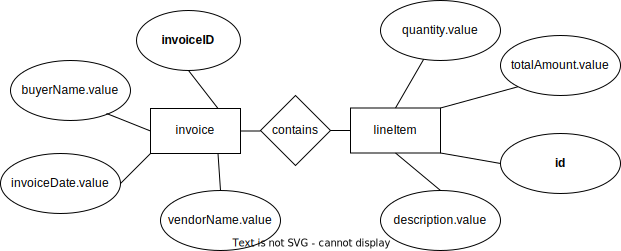
\includegraphics[height=5cm]{Bilder/preprocessing/entity.png}
      %  \caption{Entity Relationship Diagram for Invoice Documents}
        %\label{fig:er}
%    \end{figure}
	The documents can be separated into two fundamental entities: the invoice and the line items. 
	%The entity relationship diagram (Figure \ref{fig:er}) shows how invoices and line items are related. 
	The invoice contains at least one line item, and the information in the invoice is relevant to all of its line items. This includes information about the vendor, and the invoice date. The line items of an invoice contain specific information on the products, such as the quantity and the description.
	An invoice and its line items can be matched through an unique identifier, the invoice ID, which is also the filename.
	\newpage

	 \begin{figure}[ht]
		\centering
		\includegraphics[height=11.5cm]{Bilder/preprocessing/df_schema.png}
		\caption{Theoretical Implementation of the Data Wrangling}
		\label{fig:invoice_df_schema}
	\end{figure}	

	Now, looking at the technical side of the file composition.	The data for an invoice and its line items is stored in an array of objects. The array "annotations" contains objects, each one representing information such as the invoice date or the unit price. A schematic description of how the invoice data should be represented after extraction is shown in Figure \ref{fig:invoice_df_schema}: One invoice is modeled as one row in the table. Different attributes are represented as columns.
	Information about line items have labels containing the prefix "lineItem". One invoice containing several items is represented by duplicate values of one label (in the example \ref{fig:invoice_df_schema} the label "lineItem.description.value"). Each new label "lineItem.description.value" denotes a new line item. Here, the order of the labels has to be retained during data wrangling to ensure not mixing up information about different invoice items. Each new line item should be a new row in the table of line items.
	
	The goal of the data wrangling process is to create two \lstinline|DataFrame|s, one for the invoices and one for the line items.
	Additionally, another data structure will be created to optimize recurring and complex operations.
	
	Data exploration shows, there are only 79.741 unique descriptions for the listed items. By saving only the unique values, the required space is reduced to less than one fourth compared to before. Additionally, this step is required by most machine learning models, as duplicate input values can skew the outcome. The model is chosen later, so this processing step leaves the model selection more open to different kinds of learning algorithms.
	
	After the deletion of duplicate descriptions, the relationship between one line item and its description is not one-to-one, but rather one description belonging to several different line items. Model outputs will be a classification of one description, so to restore the relationship between the classification result and one line item, a mapping is constructed.
	This dictionary (Figure \ref{fig:mapping}) maps one description to all line items (more specifically, their ID) with this description.
	\begin{figure}[ht]
		\centering
		\includegraphics[width=\linewidth]{Bilder/description_map.png}
		\caption{Mapping Descriptions to their Line Item IDs}
		\label{fig:mapping}
	\end{figure}


	After the construction of both tables and the mapping, these artifacts should be serialized. This way, they can easily be loaded into memory without the effort to reconstruct them from scratch.
	
    \subsection{Practical Implementation}
	
	The files were processed using a Python script exhibited in Appendix \ref{code:InvoiceReader}. The information on invoices is stored in a  \lstinline|DataFrame|. Worth mentioning is that some invoices contain more information than others. In this case, invoices are still appended into one table, but fields for non-existent values are left empty. In Figure \ref{fig:df-invoices}, the first invoice does not have a total amount included, but since the second one does, this column is created.
	The filename of one invoice contains the unique identifier for one invoice.
	
	\begin{figure}[ht]
		\centering
		\includegraphics[height=2.5cm]{Bilder/practical/df_invoices.png}
		\caption{Exemplary depiction for processed invoices in a DataFrame}
		\label{fig:df-invoices}
	\end{figure}

	Similarly, information on the invoice items is retrieved from the documents and stored in a \lstinline|pandas DataFrame|. Every line item has an unique id and can also be linked to the respective invoice through the filename.
	
	\begin{figure}[ht]
		\centering
		\includegraphics[height=6cm]{Bilder/practical/df_lineitems.png}
		\caption{Exemplary depiction for processed invoice items in a DataFrame}
		\label{fig:df-invoice}
	\end{figure}
	
	The resulting two \lstinline|DataFrame|s are serialized with the Python standard library \lstinline|pickle|. The data can be efficiently loaded into memory and re-serialized again with this library.
	
	This processing step allowed for storing the initial 5.12GB of data in a more usable format and takes up only a total of 393MB.

	The process of reading files from the disk is not inherently an expensive one, but in the realms of many thousand documents, processing times soon reach several days. Observing the execution of the Python code showed a peculiarity: While the utilization of the used processor was consequently at the maximum (in Figure \ref{fig:cpu} at 97.1\%), only one process is executed, leaving the total \ac{CPU} usage at only 20\%. 
	
	\begin{figure}[ht]
		\centering
		\includegraphics[height=5cm]{Bilder/practical/python_processes.png}
		\caption{\acs{CPU} Usage during single-process Python Execution}
		\label{fig:cpu}
	\end{figure}
	
	
	One question that may now arise is: Why doesn't Python split up the workload and employ the full capacity of the machine?
	This can be explained with the design of the Python interpreter. The Global Interpreter Lock controls access to the Python Virtual Machine executing the code. This lock only allows exactly one thread to run at a time \cite[ch.~18.3.1]{corePython}. This of course is not favorable, as valuable CPU capacity is idle. Fortunately, the lock behaves in a special way regarding C routines: the lock is released before executing C code \cite[ch.~18.3.1]{corePython}. I/O operations in Python, such as opening files, utilize C code. This allows to bypass the, in this case, inconvenient locking mechanism. 
	
	Different Python libraries exploit this specialty and allow to spawn a pool of different processes, which then execute calls asynchronously. The \lstinline|ProcessPoolExecutor| is one example of multiprocessing.
	
\begin{lstlisting}[language=python, 
label=code:process-pool,
caption=Spawning a Process Pool in Python,
style=EigenerPythonStyle]   
with concurrent.futures.ProcessPoolExecutor() as executor:
	results = process_map(r.read_invoice, filenames, chunksize=2000)
\end{lstlisting}

	The \lstinline|ProcessPoolExecutor| (s. listing \ref{code:process-pool}) can distribute a list of input values for functions onto a function. Additionally, the \lstinline|chunksize| as parameter specifies how large the bundles of input values for each process are. Distributing the workload onto all \ac{CPU} cores, the processing time was reduced from 27 hours to under 4 minutes. 
	
	\section{Data cleaning}
	Data cleaning concerns removing all impurities from the data. This includes deleting duplicates, using an uniform data type, and removing unnecessary information.
	Just the descriptions of all the line items will be fed into models, therefore only those have to be cleaned. The Python library \ac{NLTK} provides useful methods for cleaning textual data.
	
	\lstinputlisting[
	label=code:cleaner,    % Label; genutzt für Referenzen auf dieses Code-Beispiel
	caption=Python Script for extracting JSON Data into a DataFrame,
	captionpos=b,               % Position, an der die Caption angezeigt wird t(op) oder b(ottom)
	style=EigenerPythonStyle,   % Eigener Style der vor dem Dokument festgelegt wurde
	firstline=0,                % Zeilennummer im Dokument welche als erste angezeigt wird
	lastline=23                 % Letzte Zeile welche ins LaTeX Dokument übernommen wird
	]{Quellcode/cleaner}
	
	In the code example \ref{code:cleaner}, the text is firstly separated into tokens. Then each token is examined whether it contains non-alphabetic characters. Only alphabetic tokens are retained. Again, this process is highly computationally intensive due to the size of the data. Therefore, this task was completed using the same procedure for multiprocessing as detailed in the prior section.
	
\begin{lstlisting}[
	language=sh,
	caption=A Description before and after Data Cleaning,
	label=code:cleaned_descr
	]
$ python3 -c 'import cleaner; print(cleaner.clean("500grams of special baking flour type 504"))' \\
>>>  ['of', 'special', 'baking', 'flour', 'type']
\end{lstlisting}
	 
	 The code example \ref{code:cleaned_descr} shows the input and output of this procedure. A token is completely discarded if it contains non-alphabetical characters, as these tokens are more than often not an accurate descriptor of the text's meaning.	

        
        \section{Feature Extraction and Feature Engineering}
        \label{section:feature-extraction}
        The majority of popular \ac{ML} algorithms require the input of scalar, vector or matrix data. The following sections discuss alternatives for feature extraction.
            \subsection{Alternatives}
            Firstly, the distributional representations will be explained and evaluated.
            
            \subsubsection{Term-Document Incidence Matrix}
			\label{section:tdim}
            \begin{figure}[h]
            	\centering
            	 \includegraphics[height=3.5cm]{Bilder/corpus_bow.png}
            	\caption{Example Corpus}
            	\label{fig:term-doc-incidence}
            \end{figure}
            The three documents in Figure \ref{fig:corpus} will be considered to explain the workings of the one-hot encoding. A corpus is transformed into a term-document incidence matrix representation in two steps. 
            
            \begin{figure}[h!]
            	\centering
            	\includegraphics[height=2.5cm]{Bilder/preprocessing/term-document-incidence.png}
            	\caption{Term-Document Incidence Matrix}
            	\label{fig:corpus}
            \end{figure}
            
            Firstly, the vocabulary is determined. 
            It is a collection of all words occurring in the corpus. Every word is contained exactly once, regardless of the actual number of occurrences. The vector representation of one document is of the same length as the vocabulary. One document being represented by one vector, a corpus of several documents can be represented as a matrix. The resulting matrix $M$ has the size $ |D|*|V| $, with $|D|$ being the number of documents in the corpus, and $|V|$ being the size of the vocabulary.
            
            Secondly, for each combination of one document $ d_{i} $ and one word $ v_{j} $ in the vocabulary, it is determined whether the word occurs in the document. This information is encoded binary with a "1" at $m_{ij}$ for occurrence and a "0" for no occurrence. The resulting vectors for the three documents are:
            \[ d_{1} = [0,1,0,0,0,1,0,0] \]
            \[ d_{2} = [1,0,1,0,1,0,1,1] \]
            \[ d_{3} = [0,0,0,1,0,0,0,1]\]
    		The drawback of this method is that no consideration is paid to words being repeated in one document. Additionally, no semantic relationship between words or documents can be inferred. 
    		Further, it can be stated, that the \ac{BoW} representation fails to capture the meaning of synonyms. This becomes obvious with an example: document $ d_{1} $ and $ d_{3}$ would be considered to belong into the topic of transportation or automotive. The \ac{BoW} representation suggests topical proximity between document $ d_{2} $ and $ d_{3}$ , through the shared word "ticket". "Ticket" here is used in both the meaning of an entrance pass ($d_{2}$) and in the meaning of a note for a traffic offense  ($d_{3}$). 
    		Further, this feature extraction method strongly suffers from high dimensionality \cite[ch.~3.2]{practicalNLP}, since the matrix dimensions depend on the size of the vocabulary. 
    
            \subsubsection{Bag of Words Model}
 			With the \ac{BoW} model, the only difference to a term-document incidence matrix is that the occurrences of a word are counted, instead of a binary encoding.
             \begin{figure}[ht]
            	\centering
            	\includegraphics[width=\textwidth]{Bilder/bow.png}
            	\caption{\acl{BoW} Representation of Documents}
            	\label{fig:bag-of-words}
            \end{figure}
            
            The result of vectorization are three vectors:
            \[ d_{1} = [0,1,0,0,0,1,0,0] \]
            \[ d_{2} = [1,0,1,0,1,0,1,2] \]	
            \[ d_{3} = [0,0,0,1,0,0,0,1]\]
            
            \subsubsection{Tf-Idf}
            \label{section:tfidf}
            The \ac{TF-IDF} model aims to capture more meaning from the corpus by considering the composition of the whole corpus for the calculation of individual document vectors. \ac{TF-IDF} makes two assumptions about natural language:
            \begin{enumerate}
            	\item A word $t_{i} $ which occurs very frequently in one document is considered to describe a text very well (term frequency).
            	\item A word $t_{i} $ which occurs in a large number of documents does not describe one document well (inverse document frequency).
            \end{enumerate}
            
            \subparagraph{Term Frequency}
            The occurrences of one word in one document is denoted as $ \#( t_{i}) $.
            One additional consideration needs to be made regarding the document length. In a document of length $ |d_{2}| = 6 $ and a document of length  $ |d_{3}| = 2 $, the word $ t_{i} $occurring once should be considered more important to $ d_{3} $, since it accounts for a larger share of the text. The measure resulting from this idea is the term frequency:
            
            \[ TF(t_{i}, d_{j}) =   \dfrac{\#( t_{i})}{|d_{j}|} = \dfrac{occurrences \; of \; word \; t_{i} \: in \; document \;\:   d_{j}}{length \; of \; d_{j}} \]
            
            \subparagraph{Inverse Document Frequency}
            Words occurring in many documents often are articles or pronouns (stop words) which do not provide value when inspecting the content of a text. The inverse document frequency is a measure accounting for this fact. The inverse document frequency of a word is the proportion between the number of documents in the corpus and the number of documents containing the word. The logarithm is applied, as the importance of a word does not increase proportionally to the number of occurrences.
        
            \[ IDF(t_{i}, d_{j}) = \log \dfrac{|D|}{\#(d_{t_{i}}) } =  \log \dfrac{number \;  of\;  documents \;  in \; corpus \; D}{ number \; of \; documents \; containing \; word \; t_{i}} \]
            
            Combining both assumptions, the \ac{TF-IDF} measure is created:
             \[ TFIDF(t_{i}, d_{j}) \;=\; TF(t_{i}, d_{j}) * TF(t_{i}, d_{j})\]
            
            For the corpus displayed in the previous section the document vectors calculated with the \ac{TF-IDF} measure are:

           \begin{table}[!ht]
           	\centering
           	\begin{tabular}{llllllllll}
           		$d_1 = [$ & 0.     & 0.7071 & 0.     & 0.     & 0.     & 0.7071 & 0.     & 0.     & $]$ \\
           		$d_1 = [$ & 0.3979 & 0.     & 0.3979 & 0.     & 0.3979 & 0.     & 0.3979 & 0.6053 & $]$ \\
           		$d_1 = [$ & 0.     & 0.     & 0.     & 0.7959 & 0.     & 0.     & 0.     & 0.6053 & $]$
           	\end{tabular}
           \end{table}
                
            The \ac{TF-IDF} measure corrects some of the pitfalls of the \ac{BoW} model. It certainly is less vulnerable to skewing by stop words,  as words are ranked by importance to each document and the all over corpus. 
            
        
            The above mentioned methods are distributional representations \cite[ch.~3.3]{practicalNLP}. They all suffer from similar problems. The vectors contain one element for each word in the vocabulary, resulting in vectors which are high-dimensional and very sparse. Also, \ac{TF-IDF} fails to represent the topical relationship between $ d_{1} $ and $ d_{3}$. Finally, these methods can not handle an inference for words which are not in their vocabulary \cite[ch.~3.2]{practicalNLP}.
            
            Following methods are distributed representations. They are designed to alleviate the drawbacks of distributional word representations.
            
            \subsubsection{Word Embedding BERT}
             The most desirable vector representation consists of dense low-dimensional vectors which are close to each other if the words are considered similar. The lack of understanding of related words, and the problem of high-dimensionality is corrected with the third presented option: word embeddings.
            
            An embedding is a translation of a word into a high-quality vector. The model does so, as it has been trained on a large set of natural language data. The first model for continuous vector representations was word2vec \cite{word2vec2013}. Being published in 2013, the model has been already replaced by new state-of-the-art models such as \acs{BERT}. This new model builds on the premised of word2vec, but was able to obtain astonishing results at tasks such as answering questions using the Stanford Question Answering Dataset \cite[p.~6]{BERT}. 
            
            The \ac{BERT} model can represent unlabeled text by learning on large textual corpora. Its name is assembled from its different components:
            
			\begin{table}[!h]
				\begin{tabular}{lll}
					\vspace{0.5cm}
					B & Bidirectional   & \begin{tabular}[c]{@{}l@{}}The model considers both left context (previous words) and \\ the right context (following words) during learning.\end{tabular}        \\
					\vspace{0.5cm}
					E & Encoder         & The model consists of several encoder layers.                                                                                                                     \\
					\vspace{0.1cm}
					R & Representations & \begin{tabular}[c]{@{}l@{}}Sequence representations are a projection of a sequence \\ onto a vector which is able to reflect the sequence's meaning.\end{tabular} \\
					\vspace{0.1cm}
					& from            &                                                                                                                                                                   \\
					\vspace{0.1cm}
					T & Transformers    & \begin{tabular}[c]{@{}l@{}}BERT belongs into the family of transformer models and \\ utilizes parts of the transformer architecture (see Figure \ref{fig:transformer}).\end{tabular}                
				\end{tabular}
			\end{table}

           
           The model is trained on two tasks. Firstly, it is trained on word prediction (see Figure \ref{fig:mlm}). \ac{BERT} had to predict one missing word in a text unit. The objective of course is to get the right word. The loss in this task is measuring if and how wrong a prediction is. The second task is to predict the next sentence after a text section. The objective is to predict the correct words and their order. The model is trained by adjusting internal weights in such a way, that both losses are minimized. In turn this means, the model can predict missing words and next sentences with minimized error.
           
          
             \begin{figure}[h!]
             	
             	\centering
             	\includegraphics[height=10cm]{ Bilder/preprocessing/BERT/BERT-language-modeling-masked-lm.pdf}
             	\caption[Training BERT with the MLM task]{Training BERT with the MLM task \cite{alammarIllustratedBERTELMo}}
         		\label{fig:mlm}    
         \end{figure}
            
         
               BERT is trained with millions of Wikipedia articles, meaning the inputs is a large text database. The text segment is split into tokens, which are then encoded as a vector of length 768 \cite[p.~3]{BERT}. Next follows the positional encoding. When applying the transformer encoder to a sequence of words, the output should be dependent of the sequence of the input words. E.g. the sentences "Bob is taller than Alice" and "Alice is taller than Bob" should be encoded as two different vectors. This can be realized with encoding the position of each token. 
               

               
               The token embedding and its positional encoding are now added, and fed into the encoder \cite{illustratedTransformer}. Inside the encoder, four elements process the input sequentially:
               
               \begin{enumerate}
               	\item The self-attention mechanism allows for the model to incorporate the context of a token into its encoding. The mechanism does so by calculating the importance of inputs with themselves ("self") and returns which tokens are important to each other's meaning ("attention").
               	\item To reduce the computational requirements for training a deep neural network, the layers of neurons in the networks are normalized with respect to their activation. This reduced the training time while not impacting the result, which is only dependent on the learning algorithm \cite[p.~10]{baLayerNormalization2016}.
               	\item The \ac{FFNN} takes the results of the layer normalization and the residual connection as input. When the whole transformer is trained on a specific task, the parameters (weights) of this model are also trained. Therefore, the \ac{FFNN} is one gear in the whole process of reaching the transformer's task.
               	\item Finally, the results are normalized again.
               \end{enumerate}
       			
%       			 \begin{figure}[h!]
%       				
%       				\centering
%       				\includegraphics[height=7cm]{Bilder/preprocessing/BERT/encoder.png}
%       				\label{fig:encoder}
%       				\caption[The Transformer Encoder Architecture]{The Transformer Encoder Architecture  \cite{illustratedTransformer}}
%       			\end{figure}
			
            
            Evaluating all different models for word vectorization, BERT clearly outperforms the distribustional representations:
            \begin{itemize}
            	\item Word embeddings produce dense and lower-dimensional vectors than distributional representations.
            	\item With word embeddings, the resulting vectors perform a lot better on common \ac{NLP} tasks, meaning the resulting vectors are of higher quality than with distributional representations.
            	\item BERT can process out-of-vocabulary words, this is a big advantage to previous embeddings.
            \end{itemize}

			The advantage of BERT over the other presented options is obvious. But, now there are two unconsidered restrictions:
			First, BERT only encodes words.
			Second, BERT can only handle one language.
			
			Luckily, researchers around BERT encountered similar tasks and developed a new BERT model to solve this. 
			First, the Sentence-BERT embeddings are generated in a way that requires only minimal additions to the BERT architecture \cite[p.~2]{sentenceBERT}. Sentence-BERT is trained with a dataset of sentences, labeled with their relationship (contradiction, entailment, neutral) \cite[p.~4]{sentenceBERT}. Two sentences each pass through a BERT model. A pooling layer for each of the two calculates a weighted sum of all words in the sentence to create the embedding for the whole sentences. With the labels and the comparison of two sentence embeddings, the pooling layer is trained. The weights in both pooling layers are adjusted over time, creating a so-called Siamese Network.
			
			Secondly, the embeddings need to be able to understand different languages. A multilingual implementation of BERT can solve this. A multilingual embedding should align vectors in different languages in such a way, that translated sentences are very close in the vector space. A multilingual Sentence-BERT model trains on a dataset with sentences and their translation \cite[p.~2]{mBERT}. The weights in the BERT model are adjusted by completing the task of assigning the same sentence in different languages a similar vector \cite[p.~2]{mBERT}.
			
			Both the multilingual and sentence embeddings require very little additional complexity compared to the underlying BERT model. But, these additions help to accurately represent the content in the dataset.
			
            \subsection{Theoretical Implementation}
            
           	After explaining and evaluating the alternatives, the most favorable one, the word embeddings using \ac{BERT} will be put into practice. In theory, a BERT model would have to be trained using a large text dataset. This took the developers of BERT at Google 4 whole days, and required 4 \ac{TPU}s \cite{BERTTraining}. Fortunately, the researchers published this trained model, making it free to use for the public \cite[p.~2]{BERT}.
            	
            From the available pre-trained models, the \lstinline|distiluse-base-multilingual-cased| model fulfills all the requirements (sentence embeddings, multilingual vector alignment). The prefix 'distiluse' stands for distilled universal sentence encoder, meaning the sentence encoder is compressed in a model with a more portable size. The suffix 'cased' means that words are handled case-sensitive.
            
            Since the description data has already been transformed into a usable format and cleaned, the descriptions can now easily be fed into the \lstinline|distiluse-base-multilingual-cased| model.
            	
            \subsection{Practical Implementation}
             
             The model can be loaded using the library \lstinline|sentence_transformers|. The library can create a model from the name of the transformer. Embeddings can be generated very easily, and are returned as a 2D-array. This inference takes about 30ms. For all 79.741 documents, this means an total time of about 40 minutes.
             
\begin{lstlisting}[language=python,
	label=code:generate-embed,
	caption=Generating an Embedding with BERT,
	style=EigenerPythonStyle]   

from sentence_transformers import SentenceTransformer
model = SentenceTransformer(
	'sentence-transformers/distiluse-base-multilingual-cased-v2'
	)
sentence = ["Service Charge for Flight FRA-LAX"]
embedding = model.encode(sentence)
print(embedding)
>>> 	[[-0.02105838 -0.01305696 -0.0403975  ...  0.08315323  0.06774105  0.03354893]
\end{lstlisting}

		Since data cleaning and data wrangling could be sped up significantly with multiprocessing, it stands to reason that this might also work for the inference on BERT. Batching and parallel processing only provides a speed-up if the model can utilize a strong \ac{GPU} \cite{schopfParallelInferenceHuggingFace2022}. This is not the case, so we settle with a one-time processing taking 40 minutes.
		
		During processing, the hardware was overheating and shutting down. To prevent losing progress, batches of 1000 documents were processed at a time, serialized and written on the hard disk. Upon completion, the files are loaded into memory again and unified into one collection of 20MB in vectors.

		These vectors are now ready for clustering.            
\chapter{Modelling}
The objective of this thesis is the grouping of expenses with the methods of \ac{NLP}. Grouping, or clustering, is the practise of sorting data points into groups in such a way that the similarity inside a group (intra-cluster similarity) is high while the similarity between clusters (inter-cluster similarity) is low. The defintion of similarity as well as different clustering algorithms are presented and contrasted in the following sections.

\subsection{Similarity and distance measures}
A distance measure is a quantification of how near objects in space are. Distance measures can be defined for spaces of arbitrary numbers of dimensions. 



\subparagraph{Euclidean Distance} \label{euclidean}
The most intuitive and popular distance measure is the euclidean distance. This measure is applicable for vector spaces $F^{n}$ with $n \in \mathbb{N}_0 $. For low-dimensional applications, this distance works well and shows great results. Euclidean distance can be calculated in a highly efficient manner, even for n dimensions. This suggests, that euclidean distance is particularly suitable for high-dimensional data. Unfortunately, euclidean distance falls victim to the curse of dimensionality. In \cite{beyerNearestNeighbor} it is proven that with increasing dimensions, the distance between data points approaches an uniform value for all datapoints. This effect could be demonstrated for spaces with as little as ten dimensions. Therefore, it can be said that euclidean distance is not suitable for high-dimensional data. With vectors in \ac{NLP} ranging from 100 to 800 dimensions, this distance measure is not suitable.

\subparagraph{Dot Product}


\subparagraph{Cosine Distance}


\subsection{K-Means with Euclidean Distance}
\include{Inhalt/04_Inhalt/content_evaluation}

\chapter{Deployment}
	The analysis results are targeted at decision-makers such as financial analysts and strategists. The clustering results can be part of a in-depth financial analysis, and provide a very broad overview on spending.
	
	The questions this overview should answer are:
	\begin{itemize}
		\item Which spending categories exist?
		\item How does the spending divide onto the categories?
		\item Which magnitude exists between the different amounts spent?
	\end{itemize}
	
	The results of an analysis are often summarized using a business intelligence visualization tool. In this case, the analysis is visualized using Tableau.
\begin{figure}[h!]
	\centering
	\includegraphics[
	width=\linewidth,
	angle=90]{Bilder/deployment/bubble.png}
	\caption{Tableau Dashboard: Overview on the largest Spending Categories}
	\label{fig:dashboard-bubble}
\end{figure}

\begin{figure}[h!]
	\centering
	\includegraphics[width=\linewidth,
	angle=90]{Bilder/deployment/world.png}
	\caption{Tableau Dashboard: Overview on the largest Spending Categories}
	\label{fig:dashboard-world}
\end{figure}

	The dashboard answers all questions. First, it shows the big picture of spending. Additional insights are in the tool tips of each bubble in the chart. The table on the right hand side provides a convenient ranking of the different spending categories.
	







%\chapter{Discussion of Alternatives}
\section{Criteria}

\section{Data preprocessing}
- transforming json documents into dataframe rows

- removing stopwords from several languages

- removing numbers and interpunction

- tokenization

\section{Feature extraction}
\subsection{Tf-Idf}
- bag of words model
\subsection{Word2Vec, Embeddings}
- explain tf-idf
\subsection{HashVectorizer}
\subsection{n-Grams and Tf-Idf}

\section{Model}
\subsection{K-Means with Euclidean Distance}

\section{Model Evaluation}
\subsection{Elbow Diagram}

\section{Visualization}
\subsection{PCA}
\subsection{T-SNE}
%\chapter{Theoretical Implementation}

\section{Dataset selection}
Which datasets are available?


\section{Business Understanding}

\section{Data Understanding}



\section{Data preparation}

\subsection{Data processing and data wrangling}
Explain the structure of one invoice.
Explain which data structures I want to use.
\includegraphics[height=8cm]{Bilder/data_model.png}
Explain how I want to store the data. Explain the successive artifacts.

\subsection{Data cleaning}


\subsection{Feature Extraction and Feature Engineering}

\section{Modelling}
\section{Evaluation}
\subsection{Visualization}
\section{Deployment}
%\chapter{Practical Implementation}

\section{Data preprocessing}
\section{Feature extraction}
\section{Model Training}
\section{Model Evaluation}
\section{Visualization}
\chapter{Evaluation of the Result}
Different Chapters in this thesis mention their respective objectives and criteria. This Chapter evaluated the result on the basis of these standards.

\paragraph{Detailed Task Description}
The goal of this thesis is adding value to real business documents by transforming unstructured data into a structured format. The structured information can then be used as a base for further analyses.
The task is to perform a full data analysis on the supplied dataset. The dataset is to be prepared for processing with established methods. An evaluation for different means of feature extraction, machine learning, model evaluation and visualization should be performed. With the evaluation a complete flow for the data processing should be presented. The result is an added value to the dataset by creating structured data and providing insights into this data.


\paragraph{Thesis Criteria}
Section \ref{section:criteria} mentions criteria for completing the task in the corporate environment. Firstly, only available resources should be used. All calculations were completed on the already available hardware. Also, all libraries used were open-source, needing no license. Tableau is free of charge for students. Finally, no internal services were required. This criterion is fulfilled.

Secondly, the dataset required special attention with respect to data protection. The data and the extraction results were only stored on SAP-authorized hardware. Additionally, the thesis contains a restriction notice to emphasize the special caution required.

Thirdly, the solution should be designed according to industry standards. The data mining follows industry standards by using state-of-the art models such as \ac{BERT}. Also, the Tableau dashboard presents the results in a way very common to this field. The research model used is the most popular and widely-used in the industry.

Fourth, the code needs proper documentation. The Jupyter Notebook format allows for combining Python code with markdown annotations. The resulting files are a great device for telling the story of the data analysis. The code is structured using headings to signify different logical units.

Fifth, the code should be optimized in its performance. A very careful choice of data structures based on benchmarks ensures the efficiency of the source code. Storage formats like the Python \lstinline|pickle| persist the information in a memory-saving way. Also, the used parallel processing speeds up processing times.

\paragraph{Business Objectives}
The business objectives (Section \ref{section:business-objectives}) firstly specify the goal of insight into spending across different related spending. The topics generated in Subsection \ref{section:topics} summarize detailed cost into cross-cutting topics such as beverages. 


%The primary goal is the development of a solution for automatic aggregation of documents, based on topics addressed in those documents. The focus is on shorter text segments, such as product descriptions. The business objective is an information gain, on how spending is distributed among cross-cutting topics in a company.
%The created solution can be evaluated with the business success criterion: "Does the solution identify and give useful insights in the money pits?". The judgment of goal achievement is a subjective matter. Evaluating the success should therefore be distributed among several stakeholders, including but not limited to the author, the supervisor and the supplier of the data.

Section \ref{section:business-objectives} also states the clear business success criterion: "Does the solution identify and give useful insights in the money pits?". This criterion is definitely fulfilled. The dashboard clearly shows which categories take up the most funds.


\paragraph{Data Mining Goals}
The data mining goals (Section \ref{section:data-mining-goals}) are four very distinct points:
\begin{enumerate}
	\item Identifying and applying appropriate methods for feature extracting tailored to this type of dataset.
	\item Identifying and applying appropriate methods for clustering documents in this type of dataset.
	\item Identifying and applying appropriate methods for topic modeling with this type of dataset.
	\item Aggregating expenses by their clusters and visualizing the output.
\end{enumerate}


%1. Identifying and applying appropriate methods for feature extracting tailored to this type of dataset.
Firstly, the feature extraction. The part about feature extraction (Section \ref{section:feature-extraction}) presents and carefully evaluates different methods with respect to their relevance to the specific dataset. The chosen mechanism \ac{BERT} is able to fulfill all requirements, while also reflecting the current state of the art. The resulting features provide best conditions for clustering documents.

%2. Identifying and applying appropriate methods for clustering documents in this type of dataset.
Secondly, the document clustering.
%How were the methods identified?
The clustering methods are evaluated on the basis of their ability to produce meaningful clusters. 
%Which methods were this?
Both k-Means and \ac{DBSCAN} are contrasted. 
%Which method was chosen?
The k-Means algorithm is able to generate higher-quality clusters in this special domain. While \ac{DBSCAN} technically produces more clear clusters, the proximity of documents such as used in k-Means is more meaningful than being connected to each other in a high-density area.
%How good were the results?
The clusters are created with the goal of a major generalization. Therefore, in the trade off between sharp clusters (high $k$) and strong ability to generalize (lower $k$), the lowest viable number of clusters is chosen. The high quality of the results is most obvious in the very intuitive arrangement of topics in a plane (Section \ref{fig:topics}).

%3. Identifying and applying appropriate methods for topic modeling with this type of dataset.
Thirdly, the topic modeling.
% Which method for topic modeling was chosen?
The topic model generates a topic which aims to describe all documents in one cluster. The model does so by choosing three word which are highly relevant to all contained documents. 

%4. Aggregating expenses by their clusters and visualizing the output.
Fourth, the visualization.
% how are the clusters visualized
A bubble chart (Figure \ref{fig:dashboard-bubble}) shows each cluster. The size of a bubble represents the magnitude of spending in this category.
% what does the visualization tell you?
The visualization gives an easily comprehensible representation of spending. 

\paragraph{Research Questions}
%How can information from invoice-like documents be extracted? 
The thesis answers both research questions. Firstly, it presents options to extract information from invoice-like documents. With means of annotation services, careful data wrangling and data cleaning, the data is transformed into a fitting format. A language model encodes the data for further processing.Then, the data is processed with means of unsupervised machine learning. A new information is gained: there are now groups of documents which are similar to each other.

%How can extracted information provide insights?
Secondly, the extraction results provide meaningful insights by uniting the information about a group of documents with the associated cost. One can now easily see how much is spent on each group.
\include{Inhalt/04_Inhalt/Outlook}
% ---- Literaturverzeichnis
\cleardoublepage
\renewcommand*{\chapterpagestyle}{plain}
\pagestyle{plain}
\pagenumbering{Roman}                   % Römische Seitenzahlen
\setcounter{page}{\numexpr\value{savepage}+1}
\printbibliography[title=Literaturverzeichnis]

% ---- Anhang
\appendix
%\clearpage
%\pagenumbering{Roman}  % römische Seitenzahlen für Anhang
\chapter{Appendix}
\begin{table}[]
    \caption{Inventory of Resources}
    \begin{tabular}{lll}
    \textbf{Type of resources} & \textbf{Kind of resources} & \textbf{Quantification}                                                    \\
    Personnel                  & business experts           & 1 person                                                                   \\
                               & data experts               & 1 person                                                                   \\
                               & technical support          & 1 person                                                                   \\
                               & data mining experts        & 1 person                                                                   \\
    Data                       & fixed extracts             & -                                                                \\
                               & live data                  & -                                                                          \\
                               & warehoused data            & -                                                                          \\
                               & operational data           & 1 dataset                                                                         \\
    Computing resources        & hardware platforms         & \begin{tabular}[c]{@{}l@{}}1 machine \\ access to SAP AI Core\end{tabular} \\
    Software                   & data mining tools          & anaconda, jupyter                                                          \\
                               & other relevant software    & Excel                                                                     
    \end{tabular}
    \label{tabelle:inventory}
    
    *) An asterisk indicates theoretical availability of more resources, if needed.
    \end{table}

\newpage
\end{document}
